\documentclass{amsart}
\usepackage{graphicx}
\graphicspath{{./}}
\usepackage{hyperref}
\usepackage{csvsimple}
\usepackage{longtable}
\usepackage{lscape}
\usepackage{epigraph}
\title{Ethnicity Effects on Confidence in Police: Universal Human Nature Feature}
\author{Zulfikar Moinuddin Ahmed}
\date{\today}
\begin{document}
\maketitle

\section{Introduction}

Our fitting of Barndorff-Nielsen Hyperbolic Distribution fitting has succeeded sufficiently now that we can just consider inference directly from fitted parametric densities rather than the raw data.  

We are going to do this to try to establish that Confidence in Police Distribution is roughly ethnicity-independent.

\section{The Curves}

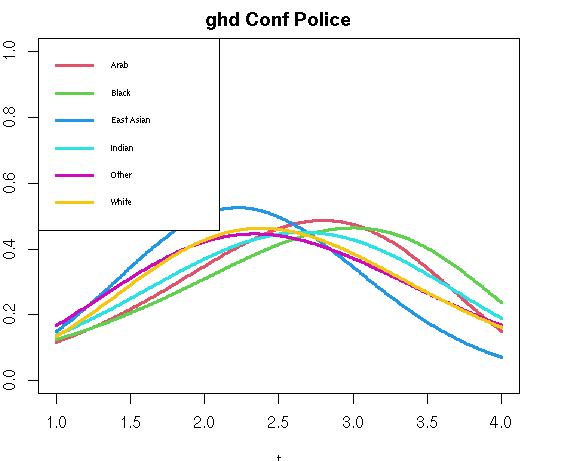
\includegraphics[scale=0.8]{cfpolice_fitted.png}

Let's take a look at the fitted Barndorff-Nielsen Distributions to understand the regularity of the curves.  We are interested here in understanding bounds on the parameters.

\pagebreak

\section{Possible Degeneracy in Fitting Parameters}

I was not aware that there could be degeracies where very different parameters yield curves that are geometrically similar.  

Let's look first at the fitted parameters.

% latex table generated in R 4.0.3 by xtable 1.8-4 package
% Tue May 18 01:05:13 2021
\begin{table}[ht]
\centering
\begin{tabular}{rlrrrrr}
  \hline
 & eth & lambda & mu & sigma & gamma & alpha.bar \\ 
  \hline
1 & Arab & -32.31 & 8.72 & 0.00 & -6.19 & 27.33 \\ 
  2 & Black & -17.77 & 7.82 & 0.00 & -5.22 & 14.27 \\ 
  3 & East Asian & -33.77 & 0.00 & 0.75 & 2.32 & 20.16 \\ 
  4 & Indian & -630.00 & 31.17 & 0.00 & -28.58 & 397.87 \\ 
  5 & Other & -12.41 & 0.00 & 0.91 & 2.61 & 8.03 \\ 
  6 & White & -13.29 & 0.00 & 0.82 & 2.64 & 8.76 \\ 
   \hline
\end{tabular}
\end{table}

Parameters for Indians is anomalous here.  Looking at curves we suspect that there is another set of parameters that will give us a fit closer to the others.

Let's just put Indians aside for the moment; we do not believe they are actually far from the rest.

Let's just take them out and compute means and stds as the rest of the fits look good.

Ah, there is a shift of weight from $\mu$ to $\sigma$ in the fits.


That's fine.  We can get geometric attribution of ehnicity effects and leave aside the parameter fits for now.

\section{Ethnicity Effects}

% latex table generated in R 4.0.3 by xtable 1.8-4 package
% Tue May 18 01:27:02 2021
\begin{table}[ht]
\centering
\begin{tabular}{rlr}
  \hline
 & eth & effect \\ 
  \hline
1 & Arab & 0.01607 \\ 
  2 & Black & 0.04307 \\ 
  3 & East Asian & 0.05944 \\ 
  4 & Indian & 0.00356 \\ 
  5 & Other & 0.00776 \\ 
  6 & White & 0.00397 \\ 
   \hline
\end{tabular}
\end{table}


\end{document}
